% arara: pdflatex
% !arara: biber
% !arara: pdflatex
% How to run: 
% 1) pdflatex "filename".tex
% 2) biber "filename"
% 3) pdflatex "filename".tex
% 4) pdflatex "filename".tex


\documentclass[x11names]{article}
\usepackage{verbatim}
\usepackage{listings}
\usepackage{graphicx}
\usepackage{a4wide}
\usepackage{color}
\usepackage{amsmath}
\usepackage{amssymb}
\usepackage[dvips]{epsfig}
\usepackage[T1]{fontenc}
% \usepackage{cite} % [2,3,4] --> [2--4]
\usepackage{shadow}
\usepackage{hyperref}
\usepackage{physics}
\usepackage{url}
\usepackage{tikz}
\usepackage{subcaption}
\usepackage[utf8]{inputenc}
\usepackage{booktabs} % Allows the use of \toprule, \midrule and \bottomrule in tables
\usepackage[font={small,it}]{caption}
\usepackage[margin=0.7in]{geometry} %Sets the margins in the document
\usepackage{siunitx}    %Allows use of SI units macros

%Defines calculator way to write powers of ten
\sisetup{output-exponent-marker=\textsc{e}}


% Change numbering and some commands
\renewcommand\thesection{Exercise \Roman{section}}
\renewcommand\thesubsection{\Roman{section}.\alph{subsection}}

%% references
\usepackage[style=authoryear,
            bibstyle=authoryear,
            backend=biber,
            % refsection=chapter,
            maxbibnames=99,
            maxnames=2,
            firstinits=true,
            uniquename=init,
            natbib=true,
            dashed=false]{biblatex}

\addbibresource{bibliography.bib}
% \addbibresource{top.bib}

% \bibliography{bibliography}
% \bibliography{top}


\usepackage[capitalize]{cleveref}

\setcounter{tocdepth}{2}

\lstset{language=c++}
\lstset{alsolanguage=[90]Fortran}
\lstset{basicstyle=\small}
\lstset{backgroundcolor=\color{white}}
\lstset{frame=single}
\lstset{stringstyle=\ttfamily}
\lstset{keywordstyle=\color{red}\bfseries}
\lstset{commentstyle=\itshape\color{blue}}
\lstset{showspaces=false}
\lstset{showstringspaces=false}
\lstset{showtabs=false}
\lstset{breaklines}


\definecolor{keywords}{RGB}{255,0,90}
      \definecolor{comments}{RGB}{0,0,113}
      \definecolor{red}{RGB}{160,0,0}
      \definecolor{green}{RGB}{0,150,0}
       
      \lstset{language=Python, 
              basicstyle=\ttfamily\small, 
              keywordstyle=\color{keywords},
              commentstyle=\color{comments},
              stringstyle=\color{red},
              showstringspaces=false,
              identifierstyle=\color{green}
              }



\title{ Exercise 4 \\ Sommerjobb Numeriske Plasmaoppgaver }
\author{Gullik Vetvik Killie	}


%%%%%%%%%%%%%%%%%%%%%%%%%%%%%%%%%%%%%%%%%%%%%%%%%%%%%%%%%%%%%%%%%%%%%%%%%%%%%%%%%%%%
% Actual text starts here
%%%%%%%%%%%%%%%%%%%%%%%%%%%%%%%%%%%%%%%%%%%%%%%%%%%%%%%%%%%%%%%%%%%%%%%%%%%%%%%%%%%%
\begin{document}


\maketitle

\section{Exercise}

\subsection{Theory}
  Starting from Faraday's law, Ohm's, Àmpere's law and the equation of motion for a infinitely conducting cold plasma, see \cref{tab:symbols} for explanation of the symbols,

  \begin{align}
    \nabla \cross \va{E} =& \pdv{\va{b}}{t} \label{eq:Faraday}
    \\
    \va{E} &= -\pdv{\xi}{t} \cross \va{B}_0 \label{eq:Ohm}
    \\
    \nabla \cross \va{b}  &= \mu_0\va{j}  \label{eq:Ampere}
    \\
    \rho \pdv[2]{\xi}{t} &= \va{j} \cross \va{B}_0 \label{eq:EOM}
  \end{align}

  \begin{table}
            \centering
            \begin{tabular}{| c | c | c |}
                 Symbol & Meaning & Value
                 \\
                 $\va{E}$ & Electric Field  & -
                 \\
                 $\va{B}_0$ & External Magnetic Field & \((4.0\times10^{11}x^{-3}, 0, 0) \si{\tesla}\)
                 \\
                 $\va{b}$ & Magnetic Field (Plasma) & -
                 \\
                 $\va{j}$ & Current Density & -
                 \\
                 $\va{\xi}$ & Plasma Displacement & -
                 \\
                 $\rho $ & Mass Density & \((50x^{2}, 0, 0) \si{\meter^{-3}}\)
                 \\
                 $ x $  & Length  & -
                 \\
                 $\mu_0 $ & Vacuum Permeability & $ 4\pi10^{-7} \si{\newton\per\ampere} $
                 \\
                 $\va{v}_A$ &  Alfvèn Velocity & $ \va{B}_0/\sqrt{\mu_0\rho}$ 
                 \\
                 $\nu$  & Plasma Spacial Displacement Velocity   & -
                 \\
                 $R_e$ & Earth Radius & $6.371\times 10^3 \si{\meter}$
            \end{tabular}
            \caption{Overview over the symbols, and values used}
            \label{tab:symbols}
      \end{table}

    Combining \cref{eq:Faraday} and \cref{eq:Ohm}, and integrating we get
    \begin{align}
      \nabla \cross \left(-\xi \cross \va{B}_0\right) &= \va{b}
      \intertext{Crossing the equation with $\nabla$ and inserting \cref{eq:Ampere}}
      \nabla \cross \nabla \cross \left(-\xi \cross \va{B}_0\right) &= \mu_0 \va{j}
      \intertext{Inserting this into \cref{eq:EOM} } 
      \pdv[2]{\xi}{t} &= \frac{1}{\mu_0\rho} \left(\nabla \cross \nabla \cross \left(-\xi \cross \va{B}_0\right) \right) \cross \va{B}_0
      \intertext{Crossing the with \(\va{B}_0\) and swapping the order of cross products we obtain}
      \pdv[2]{\va{B}_0 \cross \va{\xi}}{t} &= \va{v}_A \cross \va{v}_A \left(\nabla \cross \nabla \cross \left(\va{B}_0 \cross \va{\xi}\right) \right)
    \end{align}

    Assuming a shear and sinusoidal wave along the y-axis, \(\va{\xi} = e^{i\omega t} \va{e}_y \) this simplifies to a one dimensional wave equation with a variable cooefficient

    \begin{align}
      \pdv{\xi(x)}{x^2} &= -\xi(x) \frac{\omega}{v^2_A(x)}
      \intertext{Introducing \( \nu(x) = \pdv{\xi(x)}{t} \) we get two first order coupled differential equations}
      \pdv{\xi(x)}{t} &= \nu(x)
      \\
      \pdv{\nu(x)} &= -\xi(x)\frac{\omega^2}{v^2_A(x)}
      \intertext{Using a forward finite step we obtain}
      \xi(x + h) &= \xi(x) + h\nu(x)
      \\
      \nu(x + h) &= \nu(x) - h \frac{\omega^2}{v^2_A(x)} \xi(x)
    \end{align}

    We want to search for the standing waves on the domain \(x = [ -5R_e, 5R_e ]\), with the boundary conditions \(\xi(-5R_e) = \xi(5R_e) = 0 \si{\meter}\) and \(\nu(-5R_e) = \nu(5R_e) = 100 \si{\meter\per\second}\). Our algorithm to find the harmonic frequencies will be by trial and error, testing a frequency and then checking if it fullfills the boundary conditions, if not change the frequency and try again.

    \begin{enumerate}
      \item Define variables and constants
      \item for-loop over \(\omega\) values
        \begin{enumerate}
          \item Set initial conditions
          \item for-loop over \(x\)
            \begin{enumerate}
              \item Calculate and update $\xi(x + h)$ and $\nu(x + h)$
            \end{enumerate}
          \item Check boundary conditions \(\xi(5R_r) = 0\) and $\nu(5R_e) = \pm 100$, if true within tolerance
            \begin{enumerate}
              \item Record frequency, plot and store figures
            \end{enumerate}
        \end{enumerate}
    \end{enumerate}

\subsection{Results}
  Is there something wrong with the magnetic field, it is basically \(0\) everywhere, except at the center where it goes to infinity. I included \cref{eq:va2} to show how that causes 
  \begin{figure}
    \centering
    \begin{subfigure}{0.45\linewidth}
      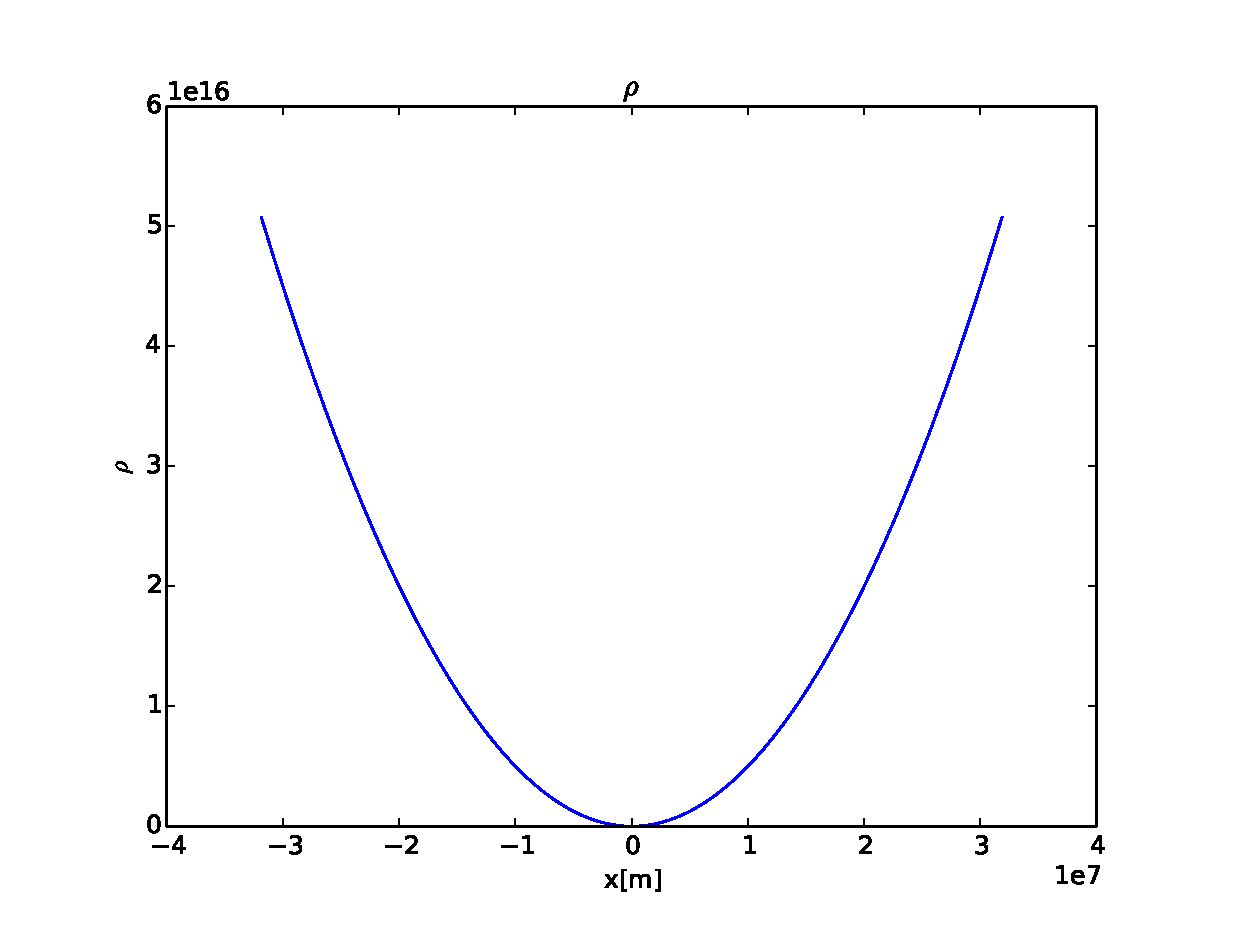
\includegraphics[width = \textwidth]{figures/rho}
    \end{subfigure}
    \begin{subfigure}{0.45\linewidth}
      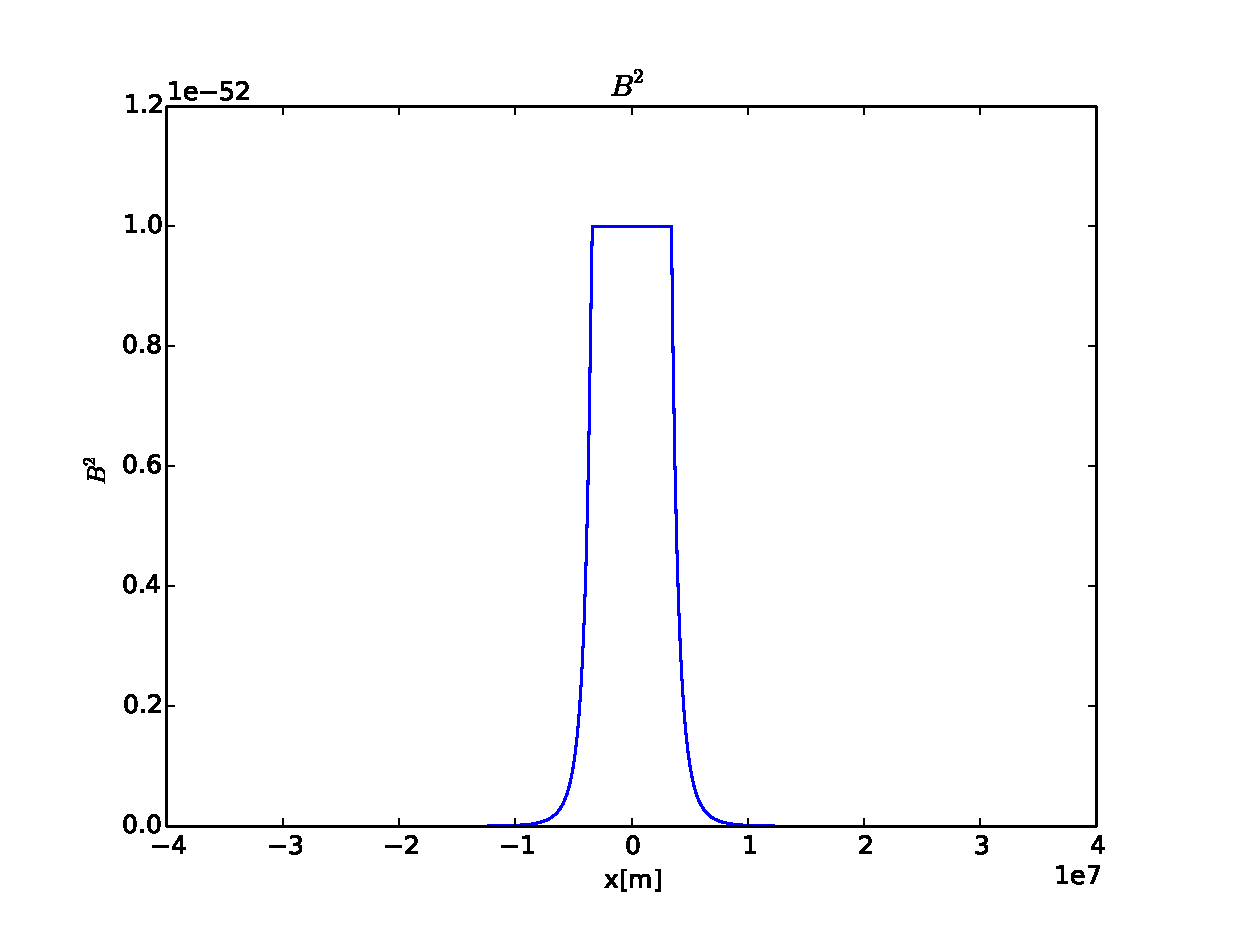
\includegraphics[width = \textwidth]{figures/b2}
    \end{subfigure}
     \begin{subfigure}{0.45\linewidth}
      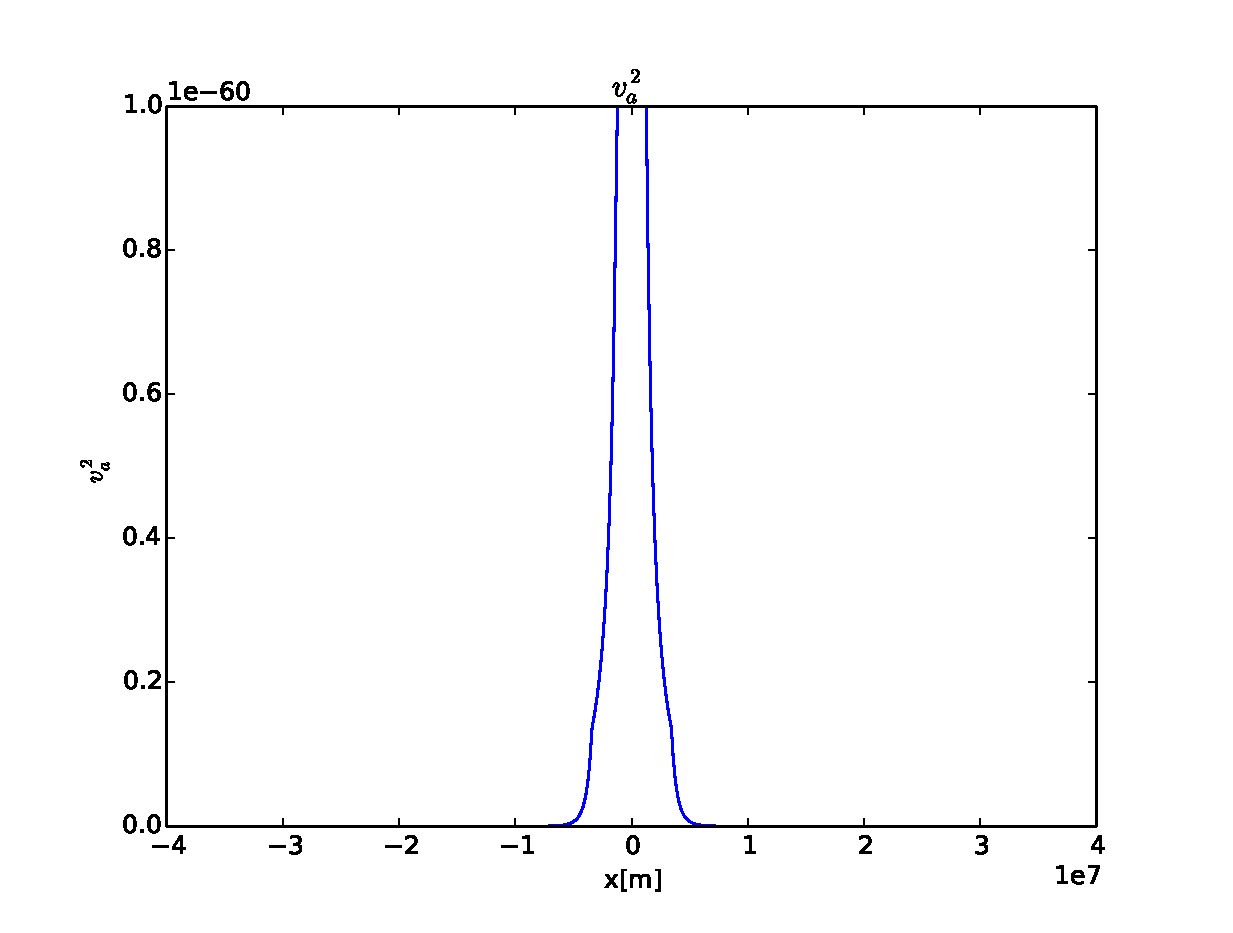
\includegraphics[width = \textwidth]{figures/va2}
    \end{subfigure}
    \begin{subfigure}{0.45\linewidth}
      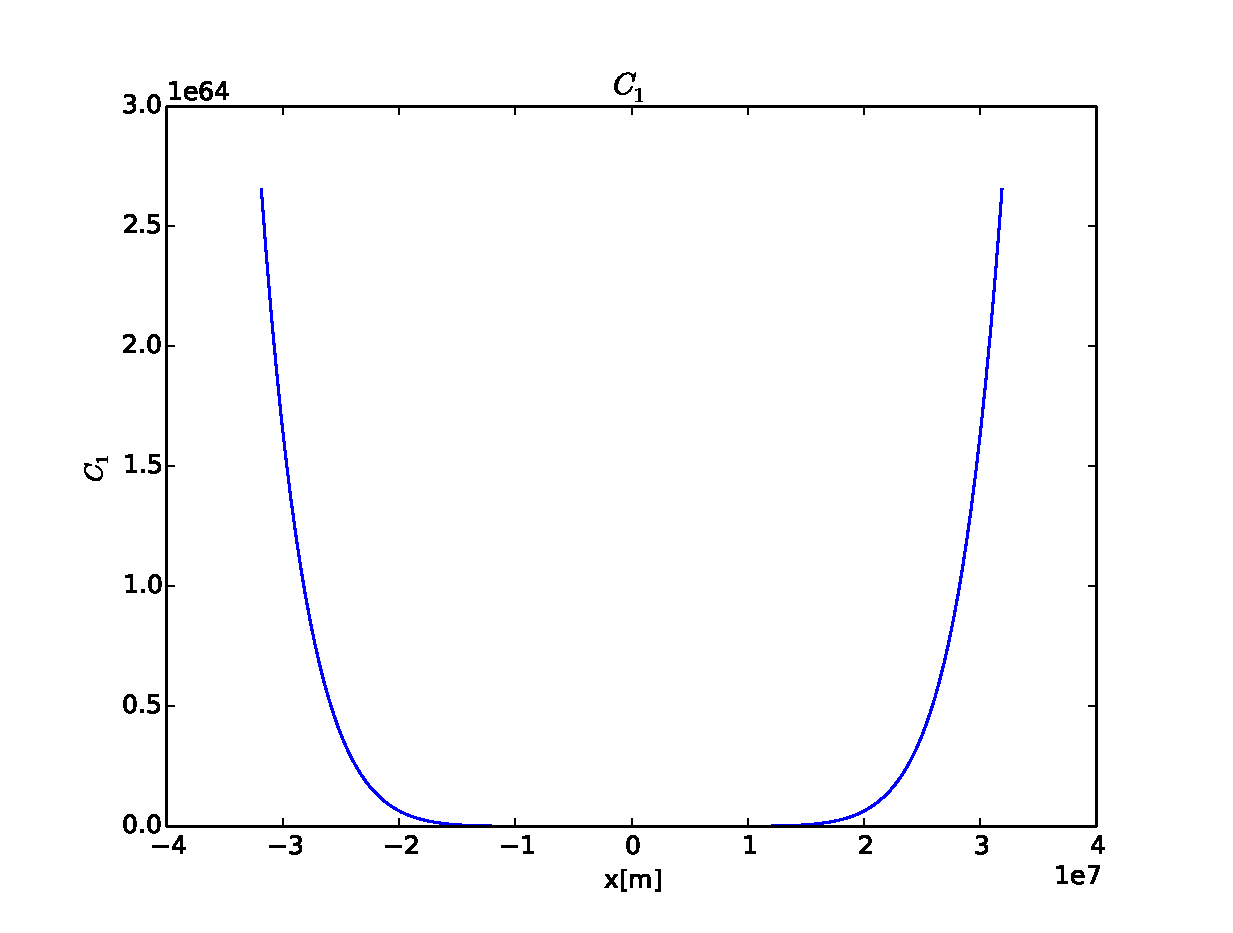
\includegraphics[width = \textwidth]{figures/C1}
    \end{subfigure}
    \caption{The figures show the physical characteristics that govern the wave-equation. \(\rho = 50\times x^{2}\), \(B = 400\times x^{-3} \times 10^{-9}\si{tesla}\), \(v_a^2 = \frac{B^2}{\rho \mu_0}\) and \(C_1 = h \frac{\omega^2}{v_a^2}\).}
  \label{eq:va2}
  \end{figure}

  \begin{figure}
    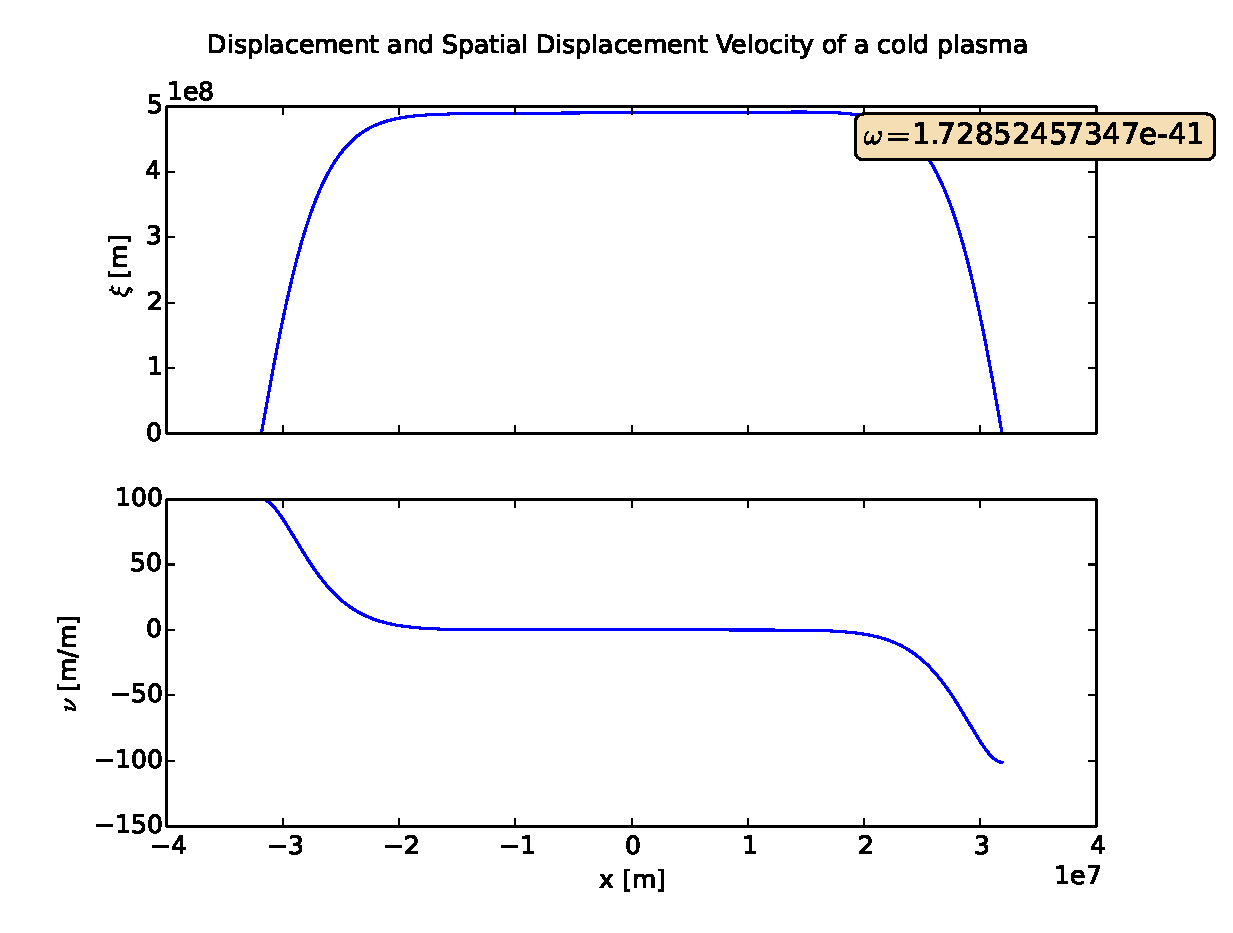
\includegraphics[width = 0.45\linewidth] {figures/wave172852}
    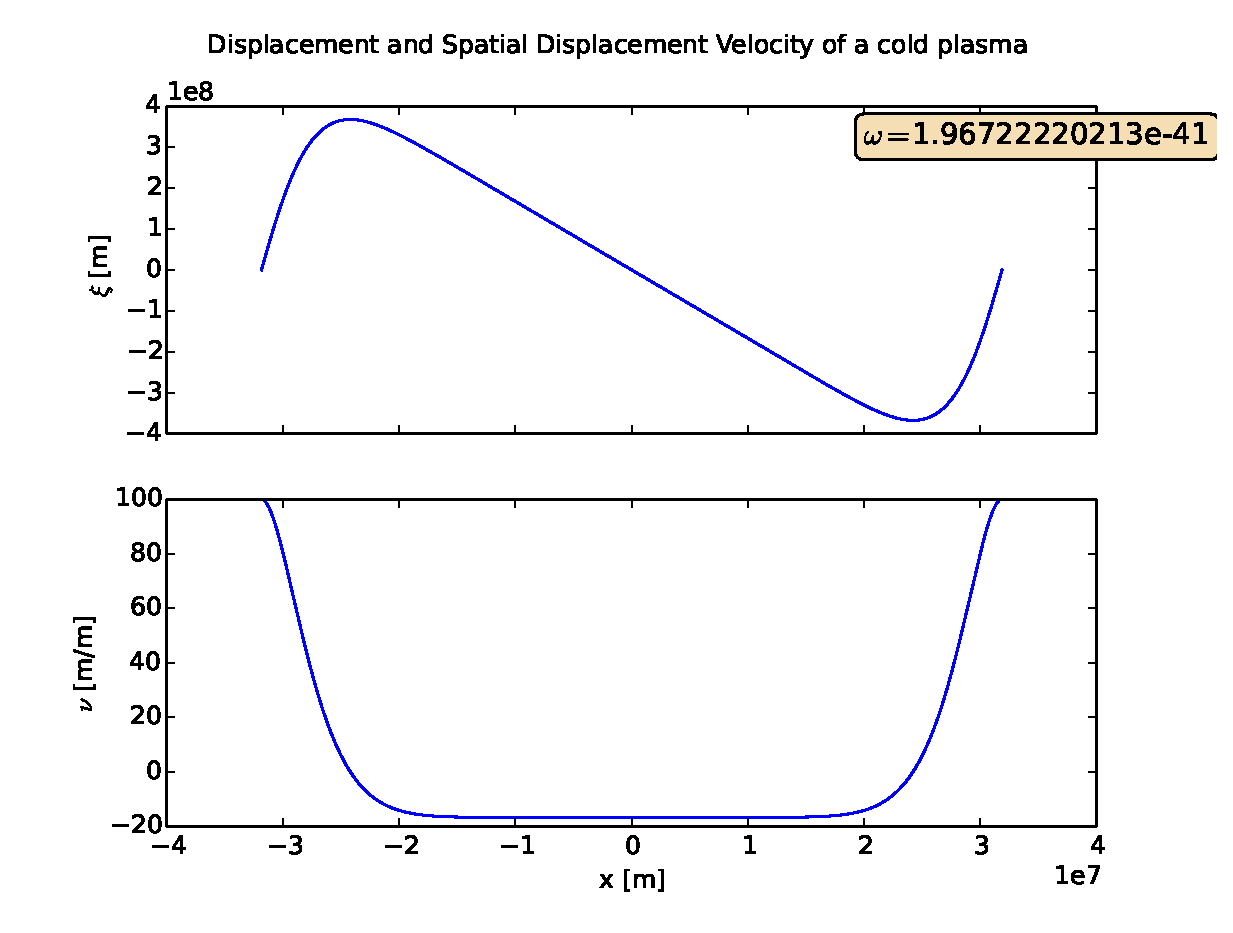
\includegraphics[width = 0.45\linewidth] {figures/wave196722}
    \caption{The first two harmonic waves, of plasma displacement, in a spatially varying magnetic field. The frequencies used are still much to low.}
    \label{fig:waves}
  \end{figure}

  We ran the simulation integrating over \(10^6\) spatial steps in the simulations, figures showing the displacement and the displacement velocity of the first two harmonics is shown in \cref{fig:waves}.
   % The first two harmonics were found at the frequencies \( \omega_1 = 1.995 \times 10^{-13} \si{\per \second} \) and \( \omega_2 = 2.765\times 10^{-13} \si{\per \second} \) and it should be noted that the second harmonic is not a integer multiple of the first harmonic, which is also true for the higher harmonics. This is because wave speed is varying over the domain.

  % The frequencies tried out had a resolution of \(\Delta\omega = 10^{-16}\), and there are some systematic uncertainties in the integration method that could cause uncertainties in the frequency values.
    
      

\appendix
\section{Comments regarding the exercise}
      \begin{itemize}
        \item Isn't it a harmonic frequency when  \(\nu(-5R_e) = 100 \si{\meter\per\second}\) and \(\nu(5R_e) = -100 \si{\meter\per\second}\) as well?
        \item At \(x = 0\) the magnetic field and mass density approaches \(\infty\), that could cause some trouble with the numerical method. I just trimmed it to a high value around \(x=0\).
          Numpy handles it by giving it by giving a really high number of the spatial mesh has a point at \(x=0\), so it works, but I think trimming it is safer if we don't want any overflow instances.
        \item I liked the find by trial and error approach. Fun way to approach the problem.
        \item The frequencies found were still low, see plots of magnetic field in Results part.
        \item The units on the boundary displacement velocities, \([\si{\meter\per\second}]\) doesn't make sense. It's x-derivative should be in length \([\pdv{\nu}{x}] = [\frac{L/T}{L}] = [T^{-1}]\), \(100\) also sounds abit high when we are covering a distance in the kilometer scale
        \item Scale of the Alfvèn velocity still seems to be iffy at the edges, causing overflow problems.
          \begin{align}
            v_A^2 &= \frac{B_0^2}{\mu_0\rho} = \frac{\left(400\times 10^{-9} x^{-3}\right)^2}{4\pi10^{-7}\times 50 x^2} 
            \\
            v_A^2 &\sim 10^{-9} x^{-8}
            \intertext{Siden x mesteparten av tiden er over 10 km,  \( x \sim 10^4\si{\meter}\)}
            v_A^2  &\sim 10^{-9} (10^{4})^{-8} = 10^{-41}
            \intertext{Som gir en typisk bølgehastighet \(C(x)\) av ordenen}
            C(x) &= \frac{\omega^2}{v_A^2} \sim  \omega^2 10^{41}
          \end{align}
        \item The relevent code for used for the the constants used is pasted here
            \begin{lstlisting}
            #Define variables
            Re = 6.371E6      #m  Earths radius
            mu_0 = 4.*np.pi*1.E-7 #N/A^2
            resolution = int(1E6) #Spatial resolution
            step = (5*Re - (-5*Re))/resolution
            omega = 1.E-41      #Hz Frequency
            magConstant = 400.E-9 #T
            densityConstant = 50.   #m^-3


            x = np.arange(-5*Re,5*Re, step)

            nu = np.zeros(resolution)      #Displacement velocity in y direction
            xi = np.zeros(resolution)    #Displacement
            b  = np.zeros(resolution)    #Magnetic field
            rho= np.zeros(resolution)    #Mass density
            vaSquared= np.zeros(resolution)    #Alfven velocity

            #Magnetic field, density and alfven velocity
            rho = densityConstant*x*x
            b   = magConstant*x**-3       #Could this also be in per cm?
            vaSquared   = b*b/(mu_0*np.abs( rho ))
            \end{lstlisting}
      \end{itemize}


\section{Code}

  \label{sec:code}
      \lstinputlisting{../source/wave.py}

      

\end{document}